\chapter{Background}
\section{Cryptocurrencies}
Before delving into the financial side of the project, it is important to understand the underlying assets and the technology that drives them.

\subsection{Blockchain}
The building blocks of cryptocurrencies come from blockchain technology. Blockchain is a distributed ledger that stores data, in blocks, in a chain, comprising the data itself as well as a full transaction history~\cite{nofer2017blockchain}. They can be thought of as a State Transition System where the state is the store of data, i.e. the owners of each token, and the state-transition function is a function of state and a transaction~\cite{ethereum_whitepaper}. The transition function defines how the transaction, $T$, should affect the state, $\sigma$. $$\sigma' = transition\_func(\sigma, T)$$Thus the state, $\sigma$, and transition function $transition\_func$ are defined by the blockchain implementation, which tends to be more complex.

\begin{figure}[!htb]
    \centering
    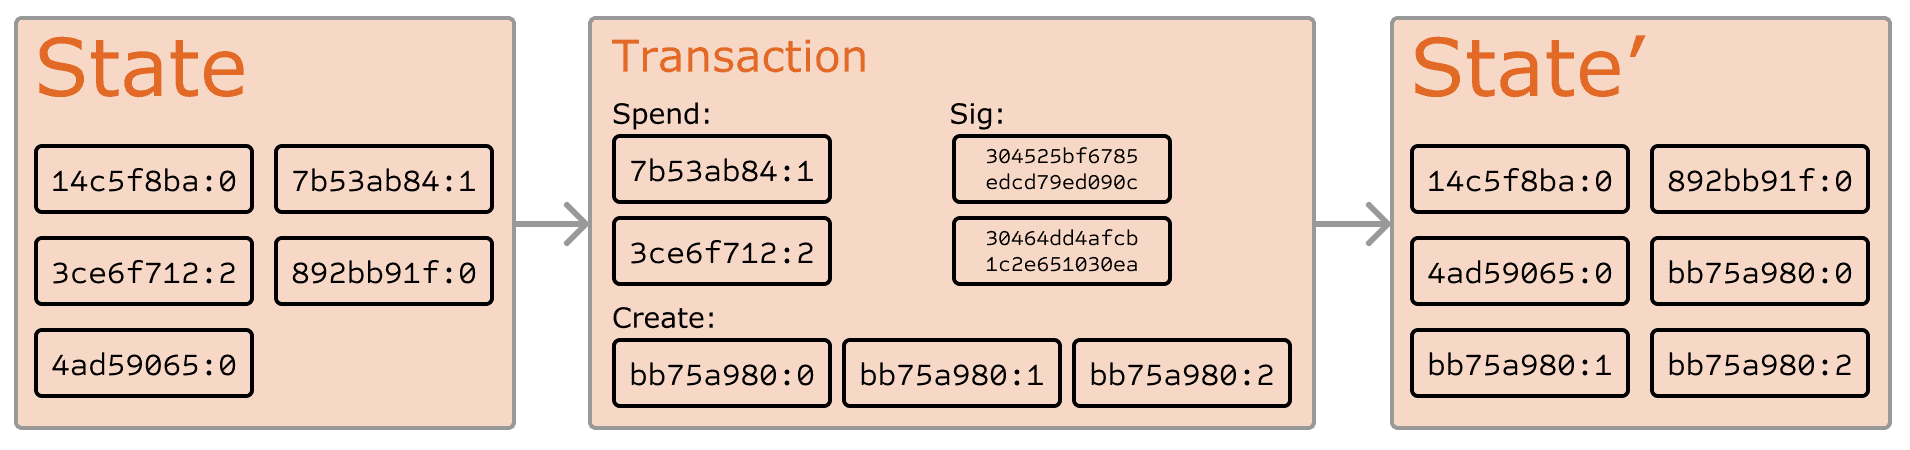
\includegraphics[width=0.8\textwidth]{background/Images/ethereum-state-transition.png}
    \caption{State Transition Diagram~\cite{ethereum_whitepaper}}
\end{figure}

\noindent In reality, a collection of transactions are batched together into a block which is then commited to the network. The components of a block can be seen below.

\begin{figure}[!htb]
    \centering
    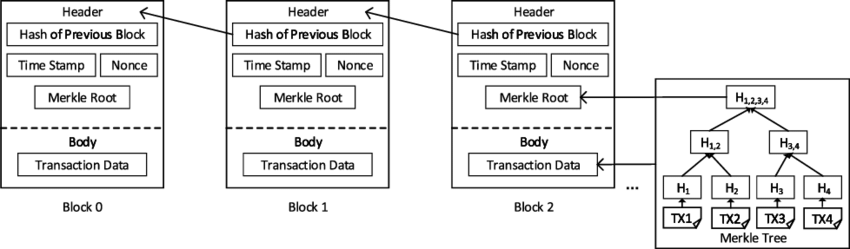
\includegraphics[width=0.8\textwidth]{background/Images/The-structure-of-a-Blockchain.png}
    \caption{Blockchain Diagram~\cite{inbookBlockchain}}
\end{figure}

\noindent A block can two significant components, the header and the body. The body of the block contains the list of transactions that are to be applied. Whereas, the components of the header may depend on the blockchain's implementation however they typically have the following key components.
\begin{itemize}
    \item \textbf{Block number} - A unique identifier assigned to each block in the chain. It serves as a chronological ordering mechanism, indicating the position of the block within the blockchain.
    \item \textbf{Timestamp} - Timestamp of the block's creation time.
    \item \textbf{Merkle Root} - A Merkle root is also stored in each block to validate transactions in the body of the block efficiently, in terms of storage and searching~\cite{noauthor_merkle_nodate}. A Merkle tree is a tree of hashes where each leaf node is its data hash and its parent node is the hash of their children's hashes. In storing the Merkle root, we do not need to directly store each transaction in each block, and also allows a quick search for any malicious alterations in differing blocks.
    \item \textbf{Hash of Previous Block} - Acts as a pointer to the predecessing block. Hence, the term ``Blockchain'' is coined as one would be able to track back to the first block from the latest block in a chain like manner.
\end{itemize}

\noindent In addition to these components, a major feature of blockchain technology is its property of being decentralised. The state of the blockchain is managed by a distributed network of nodes that are maintained by voluntary node operators. Node operators maintain the blockchain by synchorizing with the network, validating, propogating transactions and blocks and finally participating in consensus mechanisms to ensure all of the nodes agree on the current state before updating the blockchain. For this blockchain networks are typically built on a peer-to-peer (P2P) architecture. Each participant in the network, or node, has an equal status and communicates directly with other nodes. Transactions and data are shared among participants without the need for intermediaries or central servers. When transitioning to the next state, the node broadcasts the transaction, $T$, to the blockchain network and each node applies the transition function to obtain the new and same state, $\sigma' = transition\_func(\sigma, T)$. All nodes arrive to the same state as the transition function is deterministic. Once each node has applied the transition function, the network uses a consensus mechanism to the globally agreed $\sigma'$ and the transactions become actualised.
\\[3mm]
Consensus mechanisms are used to achieve agreement among participants on the validity of transactions and the order in which they are added to the blockchain. Examples of consensus mechanisms include Proof of Work (PoW), Proof of Stake (PoS), and Delegated Proof of Stake (DPoS), however current blockchains predominantly use Proof of Work or Proof of Stake~\cite{noauthor_consensus_nodate}. In addition to reaching consensus, the consensus algorithms also determine which node should be the create of a new block, which node should be granted a monetary reward.
\\[3mm]
The Proof of Work (PoW) consensus algorithm was first used in Bitcoin and is where the nodes compete to solve complex mathematical problems to verify that the transactions from a new block are valid in order to add them to the blockchain. These nodes are called miners. Once the first miner obtains the solution of the mathematical puzzle, it broadcasts the new block on the network so that the other nodes verify the solution and update their local replica. Consensus is then reaches when 51\% of the nodes agree on the new state of the blockchain. The main drawback of this algorithm is that it requires miners to perform extensive computational calculations repeatedly until they find the solution to the mathematical problem, hence once the solution has been found by a miner, after expensive work, the solution is sent along in the broadcast to the other nodes to easily and cheaply verify the solution of the problem.
\\[3mm]
To address this issue, some blockchains have opted to use the Proof of Stake (PoS) consensus algorithm as it is more energy efficient and scalable. Unlike Proof of Work, Proof of Stake use validators to create new blocks. Validators stake an amount of cryptocurrency as collatoral and the creator of a block is chosen at random from the validators, with the probability of selection based on the amount they have staked. Due to the advantages that PoS has over PoW, Ethereum has transitioned from PoW to PoS in Ethereum 2.0.

\subsection{Ethereum}
One of them was proposed by Vitalik Buterin, the co-founder of Ethereum, in a whitepaper that proposed the idea of using smart contracts to create financial products and services that could operate independently of traditional financial institutions, hence decentralised finance was birthed~\cite{buterin2014next}.

\subsubsection{Smart Contracts}
Smart contracts are programs that are self-executing contracts between buyers and sellers that deploy on a blockchain. The programs are reactive in the sense that they are only executed on the blockchain providing that certain conditions are met~\cite{noauthor_what_nodate}. These conditions are set in the lines of code in the smart contract. To posses the reactive property smart contracts are stored and executed on every participating node on the network as part of the state $\sigma$. They are also immutable and decentralised which make smart contract advantageous as they can be used to facilitate, verify, and enforce the negotiation or performance of a contract~\cite{noauthor_introduction_nodate, noauthor_smart_nodate}.

\subsubsection{Ethereum's Architecture}
Ethereum's architecture is similar to bitcoin's but has a few differences, one of which is rather than managing a distributed ledger, it uses a distributed state machine. The Ethereum Virtual Machine (EVM) defines the rules of changing states from block to block. Each node on the Ethereum blockchain contains an immutable instance of the EVM~\cite{noauthor_ethereum_nodate}.

\begin{figure}[!htb]
    \centering
    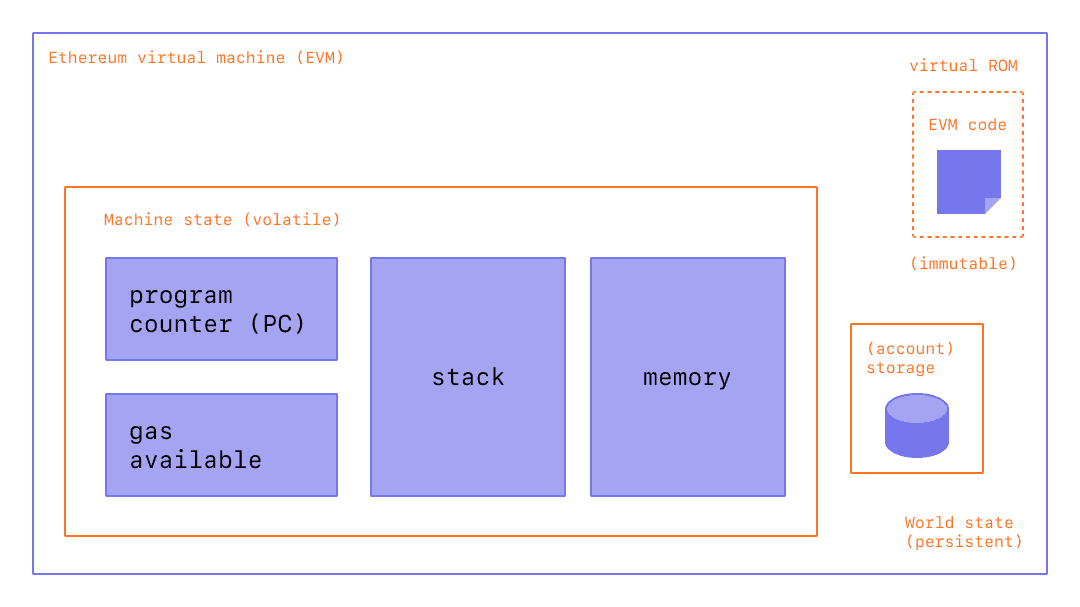
\includegraphics[width=0.8\textwidth]{background/Images/evm.png}
    \caption{EVM components~\cite{noauthor_ethereum_nodate}}
\end{figure}

\noindent Ethereum's state $\sigma$ consists of the states of all accounts where the state of an account is represented by four components: balance of ETH (the native cryptocurrency on Ethereum), a nonce, hash of the smart contract code (if account is a smart contract) and the Merkle root of smart contract storage which maintains the contracts variables (again, if account is a smart contract)~\cite{ethereum_yellowpaper}. A nonce, `Number only used once', is a number that is added to a hashed block to make the transaction more secure. It is randomly generated and used to validate a transaction. A miner first guesses a nonce and appends the guess to the hash of the current header. The miner then rehashes the value and compares this to the target hash. If the guess was correct, the miner is granted the block~\cite{noauthor_components_2021}.
\\[3mm]
Ethereum supports two types of transactions: contract creation and message calls. Message calls are used to transfer ETH from account to account and also for invoking smart contract. The process of how transactions are validated is below:
\begin{enumerate}
    \itemsep0em
    \item Validate the parent block
    \item Validate that the current timestamp is greater than the previous timestamp
    \item Check that the Ethereum concepts are valid
    \item Perform Proof of Stake on the block
    \item Check for errors and gas
    \item Validate the final state
\end{enumerate}

\subsubsection{Gas Fees}
Due to the capability of expressing loops in EVM bytecode, there is a possibility that smart contract execution could continue indefinitely. This presents a challenge as invoking a contract with an infinite loop would cause all Ethereum network nodes to become stuck executing it, resulting in a denial of service. To mitigate this issue, Ethereum has implemented a pricing mechanism. Every computation performed by a smart contract requires the payment of a fee called gas, which is denominated in ether.
\\[3mm]
To measure how much computational effort is required to execute operations on the Ethereum network, gas is used~\cite{noauthor_gas_nodate}. Every block has a base fee, derived from the demand for the block space, which is burnt. Therefore, users of the network are expected to set a tip (priority fee) to reimburse miners for adding their transaction in blocks, thus the higher the tip, the greater the incentive for miners to validate the transaction. Using gas means that the Ethereum network is tolerant to spam and also has a maximum gas fee to make Ethereum tolerant to malicious code that would be used to waste resources.

\subsection{Decentralised Finance}
One of the applications of Ethereum and smart contracts is Decentralised Exchanges (DEXes). Before delving into DEXes it is important to understand centralised exchanges.

\subsubsection{Centralized Exchanges}
Centralized exchanges(CEXes) allow agents to discover and trade assets. CEXes facilitate trading between buyers and sellers by proving an online platform that manages and maintains an order book. An order book aggregates buy and sell orders and execute matching buy and sell orders. The order book and transactions are typically managed on a central database. When trading, exchanges charge trading fees for the maker and the taker to operate the exchange and do not charge any gas fees as there is no interaction with the blockchain. 

\subsubsection{Decentralised Exchanges}
In contrast, DEXes utilize blockchain technology and smart contracts to execute trades thus providing a high level of determinism, by nature of the technology. These trades are executed on the blockchain via smart contracts and on-chain transactions. There are two types of DEX: order book DEXes and Automated Market Makers (AMMs). An order book DEX is less common and is akin to a CEX, an order book is stored on the blockchain rather than on a central database. This means each order placed requires the order book to be posted on the blockchain at each transaction. Automated Market Makers are more common and provide instant liquidity by using liquidity pools so that users can swap their tokens for a price that is determined by the portions within the liquidity pool~\cite{DEXes}. DEXes have multiple pros including lower transaction fees, privacy, diversity and trustless transactions but they also have their drawbacks such as scalability and poor liquidity a lot of the DEXes are quite new~\cite{DEXvsCEX}.

\section{Arbitrage}
Arbitrage is the process in which a trader simultaneously buys and sells an asset to take advantage of a market inefficiency~\cite{businessinsightsblog_2021}. Arbitrage is also possible in other types of securities by finding price inefficiencies in the prices of options, forward contracts and other exotics.
\\[3mm]
Sources have shown that the word ``\textit{Arbitrage}'' has been used as early as the Renaissance era when surviving documents showed a large number of bills being exchanged~\cite{poitras_2021}. There has also been some evidence to suggest that arbitrage was used as early as the Greek and Roman eras. Early forms of arbitrage would likely have been purchasing a commodity then transporting them to a foreign land and selling them at a higher price. This type of arbitrage is called commodity arbitrage and is still applicable today. With the example above, transporting the goods takes a significant amount of to the merchant, or trader, which could cause variations in the price, however, in the modern day this has been reduced and with electronic exchanges, this time to buy and sell is very small. This means inefficiencies in the market, where a trader can profit purely by buying and selling, should not exist. This is called the ``Law of One Price''. The ``Law of One Price'' states that every identical commodity or asset should have the same price regardless of exchange or location, given there are no transaction costs, no transportation costs, no legal restrictions, the exchange rates are the same and no market manipulation occurs~\cite{noauthor_law_nodate}. This is because if this were not the case, an arbitrage opportunity would arise and someone would take advantage of the scenario causing the prices on both markets to converge due to the market forces. In the real world arbitrage opportunities are tremendously common, thus allowing a risk-free investment~\cite{10.2307/1828075, RICHARDSON1978341}.
\\[3mm]
There are countless types of arbitrage such as spatial arbitrage, which profits off of different prices on exchanges in different locations, temporal arbitrage, which takes advantage of price differences at different times, risk arbitrage, which profits from perceived discrepancies in their risk-return profiles and finally market arbitrage which takes advantages of different prices on different exchanges/markets. Statistical methods include pairs trading, which involves buying and selling assets that are believed to be mispriced relative to one another, momentum trading, which identifies if assets have a strong momentum (either up or down) and profiting off of that, and finally, algorithmic trading which uses algorithms to analyze data and trades based on statistical analysis. This project shows how these opportunities can be exploited both in a pure manner as well as using statistical methods.

\section{Pure Arbitrage Techniques}
\label{sec:pure-arb}
Research into cryptocurrency arbitrage is still in its infancy and previous research has mainly focussed on the economics of cryptocurrencies, i.e. miner/trader behaviour and influence of cryptocurrency trading~\cite{eyal2015miner, avarikioti2020ride, huberman2021monopoly, athey2016bitcoin, easley2019mining, harvey2016cryptofinance, pagnotta2018equilibrium}. Furthermore, there has been very limited research comparing statistical strategies and pure methods of arbitrage of cryptocurrencies. However, it is still important to understand the basics of pure arbitrage, this form of arbitrage takes advantage of price discrepancies between three or more different currencies in the foreign exchange market. It involves executing a series of trades to profit from the imbalance in exchange rates between the currencies involved. An example of this can be seen in Figure \ref{fig:tri-arb}, given the exchange rates are \$1 = \euro 0.85, \euro 1 = \pounds0.75, \pounds1 = \$1.20, we can make a series of exchanges (trades) such that by starting with \$100, the result of this cyclic arbitrage I am left with \$130.72, hence a \$30.72 risk-free profit. Although the example uses fiat currencies (traditional currencies that are issued by governments, such as the US Dollar (USD) and the Great British Pound Sterling (GBP)), the same also holds for cryptocurrencies. Additional research into the cryptocurrency arbitrage can be found in Appendix \ref{appendix:add-background-pure-arb}.

\begin{figure}[!htb]
    \centering
    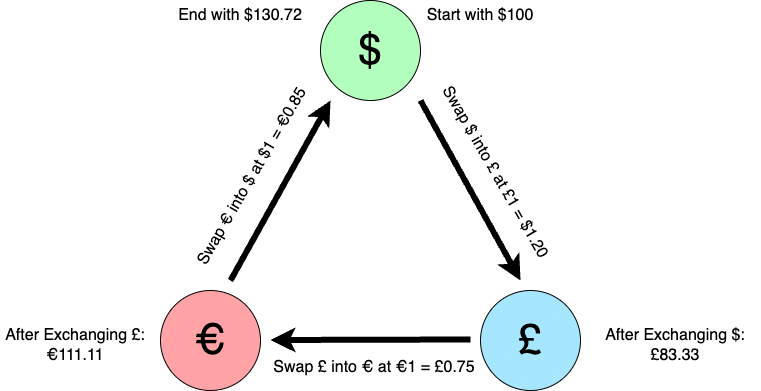
\includegraphics[width=0.8\textwidth]{background/Images/arbitrage_diagram.png}
    \caption{Triangular Arbitrage Diagram\label{fig:tri-arb}}
\end{figure}

\section{Statistical Arbitrage Techniques}
As mentioned previously mentioned and the subject of the project is to optimize statistical arbitrage methods to be able to compete with a purer form of arbitrage, i.e. cyclic arbitrage. As previously mentioned there are many methods of stat arb, pairs trading, momentum trading and algorithmic trading. Within these methods there are countless strategies to adopt and profit from, thus to limit the scope, this project I will be investigating strategies within pair trading. Research within Pair trading has been vast with many streams of approaches emerging; distance approach, cointegration approach, time-series approach, stochastic approach and some others, including using machine learning~\cite{https://doi.org/10.1111/joes.12153}. However, for this project, we will only look at cointegration/co-correlation approaches.

\subsection{Mean Reversion}
The cointegration approach follows three key steps. The first is the selection of pairs based on similarity measures, the next is assessing the tradability and finally, thresholds are set for trading. The spread is defined as $$\varepsilon_{i j,t} = P_{i,t} + \gamma P_{j,t}$$ where $P_{i,t}$ and $P_{j,t}$ denote the $I(1)$ non-stationary price processes of the assets $i$ and $j$, $\gamma$ is the cointegration coefficient, also referred to in literature as the hedge ratio. $\varepsilon_{i j,t}$ is the linear combination of the non-stationary prices and is $I(0)$ stationary and hence mean-reverting, note that stationary processes are those of which have a constant mean. Rad's implementation of this approach on stocks results in a 0.83\% return before considering transaction costs~\cite{RadLowFaff}. Another paper,~\cite{lossProtection}, looked into setting the thresholds and setting a minimum profit, $MP_{ij,t_c}$: $$MP_{ij,t_c} = \frac{n(\varepsilon_{i j,t_0} - \varepsilon_{i j,t_c})}{ \mid \gamma \mid}$$ Where $t_0$ and $t_c$ are the opening and closing times, $n$ is the volume longed of asset $j$. Additional research on the optimal portfolio designed for mean reversion can be found in Appendix \ref{appendix:add-background-opt-portfolio-des-mean-revers}.

\subsection{Statistical Arbitrage using the Kalman Filter}
Another method that is used in statistical arbitrage is using the Kalman Filter. Recall the equation for spread:
$$\varepsilon_{i j,t} = P_{i,t} + \gamma P_{j,t}$$
\noindent The Kalman filter is a recursive algorithm for estimating the state of noisy data and that needs to be filtered to be able to estimate the state of a system based on a sequence of observations, taking into account both current measurements and the system dynamics~\cite{ALSADIK2019299}. This makes it very useful to estimate the hedge ratio $\gamma$. Initially, a book by Vidyamurthy discusses best practices for choosing cointegrated equities and found that the Kalman filter was found optimal when the state-space and observation equations are linear and the noise is Gaussian~\cite{vidyamurthy2004pairs}. Since then there have been many extensions of the filter such as the Extended Kalman Filter (EKF) and Unscented KF aimed to handle when the state-space and observation equations are non-linear and the noise is not Gaussian.
\\[3mm]
The Kalman Filter works in 2 phases, prediction and update. The prediction phase is as follows $$\hat{\mathbf{x}}_k = \mathbf{F}_k \hat{\mathbf{x}}_{k-1} + \mathbf{B}_k \overset{\rightarrow}{\mathbf{u}}_k + \mathbf{w}_k$$ $$\mathbf{P}_k = \mathbf{F}_k \mathbf{P}_{k-1} \mathbf{F}_k^T + \mathbf{Q}_k $$ Where $\hat{\mathbf{x}}_k$ is the new best estimate (prediction) that is derived from $\hat{\mathbf{x}}_{k-1}$, the previous estimate and the prediction function $\mathbf{F}_k$. $\overset{\rightarrow}{\mathbf{u}}_k$ is the correction term, called the control vector, that is used when it is known that there are external influences in combination with $\mathbf{B}_k$ which is called the control matrix. In addition to this, the new uncertainty (covariance matrix), $\mathbf{P}_k$, is calculated using the previous uncertainty and additional uncertainty from the environment, $\mathbf{Q}_k $, $\mathbf{w}_k$ is called the state noise. The update is as follows $$\hat{\mathbf{x}}_k' = \hat{\mathbf{x}}_k + \mathbf{K}'(\overset{\rightarrow}{\mathbf{z}}_k - \mathbf{H}_k \hat{\mathbf{x}}_k)$$ $$\mathbf{P}_k' = \mathbf{P}_k - \mathbf{K}'\mathbf{H}_k \mathbf{P}_k$$ $$\mathbf{K}' = \mathbf{P}_k \mathbf{H}_k^T (\mathbf{H}_k \mathbf{P}_k \mathbf{H}_k^T + \mathbf{R}_k)^{-1}$$ Where $\mathbf{K}'$ is defined as the Kalman gain, $\mathbf{H}_k$ is the measurement matrix, $\overset{\rightarrow}{\mathbf{z}}_k$ is mean of the observed values, which is also calculated by $\overset{\rightarrow}{\mathbf{z}}_k = \mathbf{H}_k \hat{\mathbf{x}}_k + \mathbf{v}_k$ where $\mathbf{v}_k$ is the measurement noise, and $\mathbf{R}_k$ is the covariance of the uncertainty of the observed values~\cite{kalman_filter_bzarg}.
\\[3mm]
A paper that investigated the use of the Kalman Filter on ETFs found that the strategy it employed worked well for in-sample data points and worse, but still profitable, results for out-of-sample data~\cite{dempsey_market_2017}. The paper adapted the Kalman Filter to be able to use it for pairs trading to the following: $$\mathbf{y}_t = \mathbf{x}_t \mathbf{\beta}_t + \mathbf{\epsilon}_t$$ $$\mathbf{\beta}_t = \mathbf{I} \mathbf{\beta}_{t-1} + \mathbf{\omega}_t$$ Then calculating the Kalman Gain: $$\text{Kalman Gain} = \frac{\text{Error in the estimate}}{\text{Error in the estimate + Error in the measurement}}$$ Then to calculate the estimate: $$\text{Estimate}_t = \text{Estimate}_{t-1} + \text{Kalman Gain} \times (\text{Measurement - }\text{Estimate}_{t-1})$$ And finally, calculating the new error: $$E_{\text{estimate}_t} = \frac{E_{\text{measurement}} \times E_{\text{estimate}_{t-1}}}{E_{\text{measurement}} + E_{\text{estimate}_{t-1}}}$$ $$E_{\text{estimate}_t} = E_{\text{estimate}_{t-1}} \times (1 - \text{Kalman Gain})$$

\noindent The author states ``pairs trading strategies have gained widespread acceptance thus making profitability much more elusive'' to justify the disappointing results, however, the author fails to find evidence or provide sufficient evidence to justify the claim~\cite{dempsey_market_2017}.
\begin{figure}[htb!]
    \centering
    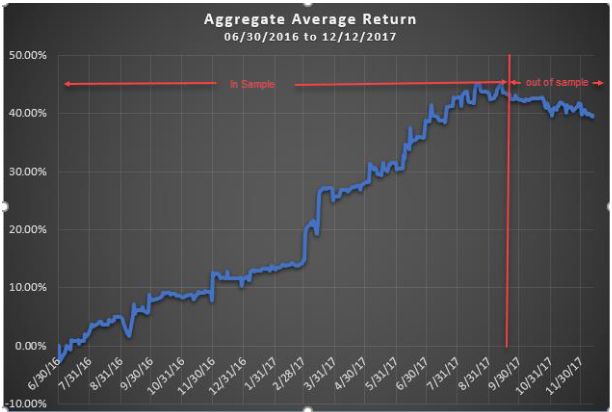
\includegraphics[width=0.9\textwidth]{background/Images/insamplevsoutsampleresults.png}
    \caption{Aggregate average return of using the Kalman filter for pairs trading on ETFs~\cite{dempsey_market_2017}}
    \label{fig:kalman_results}
\end{figure}
\\[3mm]
Another paper used the combination of the Kalman Filter and Machine Learning, more specifically Extreme Learning Machine and Support Vector Regression (SVR) to build a statistical arbitrage strategy on the Brazilian Stock Exchange~\cite{6974093}. The strategies can simply be explained as using SVR and ELM to forecast returns and using the Kalman Filter to improve the forecast.
\begin{figure}[htb!]
    \centering
    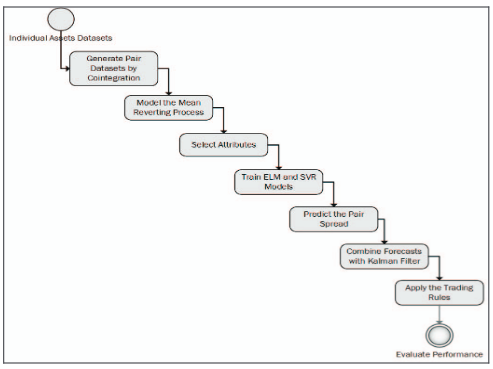
\includegraphics[width=0.9\textwidth]{background/Images/KalmanMLFlowChart.png}
    \caption{Visualisation of the trading strategy used in \cite{6974093}}
    \label{fig:kalman_ml_flowchart}
\end{figure}

\noindent The paper also compares methods, such as LASSO, BMA, and GRR, to benchmark the performance of the Kalman Filter. The research found that using simply ELM and SVR forecasts results in a return of 20.19\% and 21.32\% respectively for out-of-sample data points and using a combination with the Kalman Filter gives a return of 26.13\% for out-of-sample data points. The full results can be seen below in Figure \ref{fig:kalman_ml_results}. In addition to this, it can be seen that the volatility of the return also decreases which is ideal for investment managers.
\begin{figure}[htb!]
    \centering
    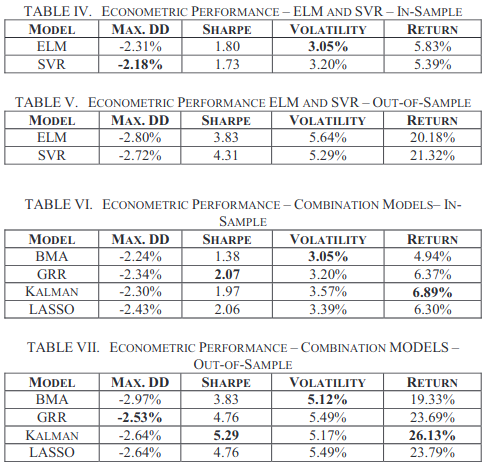
\includegraphics[width=0.5\textwidth]{background/Images/kalman_ml_results.png}
    \caption{Econometric results~\cite{6974093}}
    \label{fig:kalman_ml_results}
\end{figure}

\noindent Other papers/articles such as \cite{KRAUSS2017689, alma991000475380901591, jrfm12010031} have designed, compared and analysed other statistical arbitrage techniques using Machine Learning algorithms and revealed that some algorithms are profitable. The majority of research on machine learning trading strategies has been on assets such as stocks on centralised exchanges. The little research that has been done on statistical arbitrage on cryptocurrencies has all been on analysing arbitrage on centralised exchanges and not decentralised exchanges. One of the research projects that analysed machine learning methods of statistical arbitrage on cryptocurrencies on a centralised exchange, compared a logistic regression approach with a random forest approach~\cite{jrfm12010031}. 

%%%%%%%%%%%%%%%%%%%%%%%%%%%%%%%%%%%%%%%%%%%%%%%%%%%%%%%%%%%%%%%%%%%%%%%%%%%%%%%%%%%%%%%%%%%%%%%%%%%%%%%%%%%%%%%%%%%%%%%%%%%%%%%%%%%%%%%%%%%%%%%%%%%%%%%%%%%%%%%%%%%%%%%%%%%%%%%%%%%%%%%%%%%%%%%%%%%%%%%%%%%%%%%%%%%%%%%%%%%%%%%%%%%%%%%%%%%%%%%%%%%%%%%%%%%

% \textbf{Ones that use ML:}
% \begin{itemize}
%     \item Statistical Arbitrage in Cryptocurrency Markets \cite{jrfm12010031} %file:///home/devam/Documents/Imperial/Year_4/Individual%20Project/Interim%20Report/background/Articles/Statistical%20Arbitrage%20in%20Cryptocurrency%20Markets%20.pdf
%     \item Deep neural networks, gradient-boosted trees, random forests: Statistical arbitrage on the S\&P 500 \cite{KRAUSS2017689} %file:///home/devam/Documents/Imperial/Year_4/Individual%20Project/Interim%20Report/background/Articles/Deep_neural_networks,gradient-boosted_trees,random_forests:_Statistical_arbitrage_on_the_S&P_500.pdf
%     \item A Machine Learning based Pairs Trading Investment Strategy \cite{alma991000475380901591} %file:///home/devam/Documents/Imperial/Year_4/Individual%20Project/Interim%20Report/background/Articles/A%20Machine%20Learning%20based%20Pairs%20Trading%20Investment%20Strategy%20.pdf
% \end{itemize}

% \textbf{Broader Picture}
% \begin{itemize}
%     \item STATISTICAL ARBITRAGE PAIRS TRADING STRATEGIES: REVIEW AND OUTLOOK \cite{https://doi.org/10.1111/joes.12153} %file:///home/devam/Documents/Imperial/Year_4/Individual%20Project/Interim%20Report/background/Articles/Journal%20of%20Economic%20Surveys%20-%202016%20-%20Krauss%20-%20STATISTICAL%20ARBITRAGE%20PAIRS%20TRADING%20STRATEGIES%20REVIEW%20AND%20OUTLOOK.pdf
%     \item Statistical Arbitrage: Algorithmic Trading Insights and Techniques \cite{alma991000607977501591} %file:///home/devam/Documents/Imperial/Year_4/Individual%20Project/Interim%20Report/background/Articles/Statistical%20arbitrage%20:%20algorithmic%20trading%20insights%20and%20techniques.pdf
% \end{itemize}



% WowSwap, dydx, gmx, ... https://defiprime.com/margin-trading
% https://corporatefinanceinstitute.com/resources/cryptocurrency/cryptocurrency-exchanges/
% https://wowswap-io.medium.com/the-big-short-introducing-decentralized-leveraged-short-swaps-a81eb9d1c36f 
% https://defiprime.com/margin-trading
% https://github.com/evbots/dex-protocols
% 
% https://medium.com/defi-saver/how-to-long-or-short-any-asset-using-defi-lending-protocols-812300c9a640
% https://defiprime.com/exchanges

% https://www.youtube.com/watch?v=zABaCh3yAho - video on markovian auto regressive methods
% https://medium.com/@rachita.pateria/an-introduction-to-markov-switching-model-for-time-series-b279e9e26125

% \begin{enumerate}
%     \item \cite{HuangJianfeng2022Taaf} - %https://library-search.imperial.ac.uk/permalink/44IMP_INST/fv0fdm/cdi_informaworld_taylorfrancis_310_1080_13504851_2021_1930998
%     \item \cite{alma991000411969901591} - %https://library-search.imperial.ac.uk/permalink/44IMP_INST/mek6kh/alma991000411969901591
%     \item \cite{} - %https://library-search.imperial.ac.uk/permalink/44IMP_INST/mek6kh/alma991000343762601591
%     \item \cite{} - %https://library-search.imperial.ac.uk/permalink/44IMP_INST/mek6kh/alma996037714401591
%     \item \cite{} - %https://library-search.imperial.ac.uk/permalink/44IMP_INST/mek6kh/alma991000617323401591
% \end{enumerate}

\subsection{Analysis on Cryptocurrency Arbitrage on Centralized Exchanges}
Although the research in the papers previously mentioned does not investigate the cointegration approach on cryptocurrencies, the takeaways are the mathematical fundamentals that are used in statistical arbitrage. Kristoufek and Bouri researched the sources of stat. arb. of bitcoin in multiple centralised exchanges. The Grey correlation is built on top of the Grey system theory~\cite{JULONG1982288}, and can capture non-linear correlations without assuming a Gaussian distribution, thus using the Grey correlation provides a more robust metric to understand correlations between both series. The Grey correlation $\gamma(X_0, X_i)$ is defined with two steps:
\begin{enumerate}
    \item $\gamma(x_0(k), x_i(k)) = \frac{min_i min_k \mid x_0(k) - x_i(k) \mid + \varepsilon max_i max_k \mid x_0(k) - x_i(k) \mid}{\mid x_0(k) - x_i(k) \mid + \varepsilon max_i max_k \mid x_0(k) - x_i(k) \mid}$
    \item $\gamma(X_0, X_i) = \frac{1}{n} \sum_{i=1}^{n} \gamma(x_0(k), x_i(k))$
\end{enumerate}
\noindent With $\varepsilon \in [0,1]$, the standard is set to $\varepsilon = 0.5$.
\\[3mm]
The DCC-GARCH(1,1), \cite{engle2002dynamic}, model is also used to obtain conditional correlations for Bitcoin exchanges. The model was designed to use a combination of parameters such as the standard deviation of Bitcoin returns, traded volume, the volume of on-chain transactions, fees paid to miners, the ratio of current price and recent price history and internet hype/trends.
\\[3mm]
Upon analysis of Grey and DCC-GARCH(1,1) correlations, it is found that the DCC correlations show a little variability whereas the Grey correlations are a lot more variable ranging from 0.29 to 1. In addition, the paper then further investigates these sources and finds that these opportunities are introduced when there is a large number of inter-exchange transfer requests, i.e. the network is congested, and high price volatility. In contrast, the high volume of exchanges and on-chain activity cause the arbitrage opportunities to decrease. This paper finds and explains these sources of statistical arbitrage however does not implement or devise an algorithm that uses statistical arbitrage to generate a profit from price discrepancies of Bitcoin on different exchanges.
\\[3mm]
A paper that investigates statistical arbitrage on multiple cryptocurrencies is \cite{Figa-TalamancaGianna2021Cdff}. The authors of this paper analysed co-movements and cointegration of different cryptocurrencies on a centralised exchange using Augmented Dickey-Fuller (ADF) and  Kwiatkowsky-Phillips-Schmidt-Shin (KPSS), Ljung-Box autocorrelation tests on both stationary forms ($I(0)$) and the original form ($I(1)$). The paper then develops a dynamic factor model based on the assumption that the price dynamics of cryptocurrencies are driven by Bitcoin~\cite{blau2020comovement}, this is then evidenced by similar paths found in cryptocurrencies shown in Figure \ref{fig:pricebehaviour}.
\begin{figure}[h!]
    \centering
    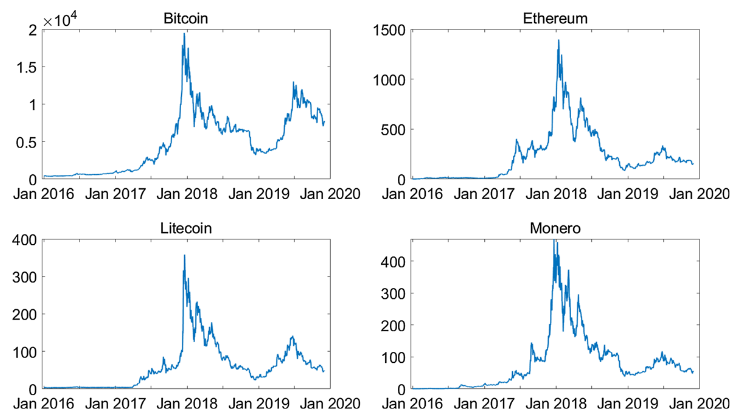
\includegraphics[width=0.8\textwidth]{background/Images/price_behaviour.png}
    \caption{Price behaviour of Bitcoin, Ethereum, Litecoin, Monero~\cite{Figa-TalamancaGianna2021Cdff}}
    \label{fig:pricebehaviour}
\end{figure}

\noindent For simplicity the authors set the number of hidden factors to 2 and upon analysis $f_1$ is a $I(1)$ process and the second factor $f_2$ is a stationary process that is independent of $f_1$. It is also found after overlaying $f_1$ with the price of Bitcoin, that the first factor strongly correlates with the price of Bitcoin.

\begin{figure}[h!]
    \centering
    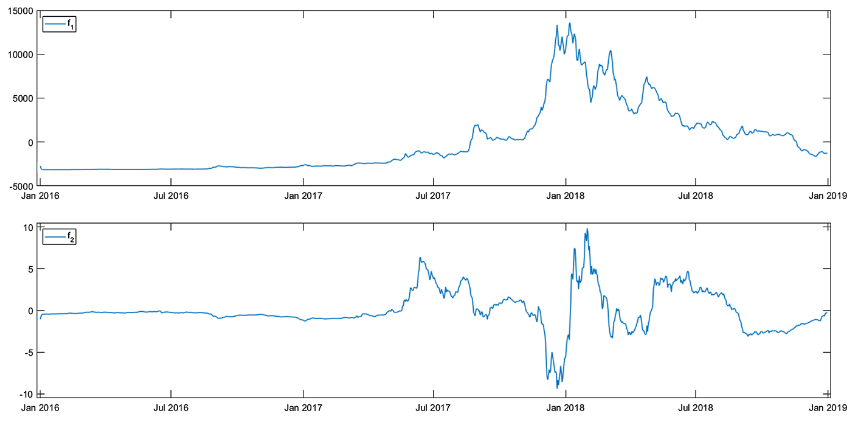
\includegraphics[width=0.8\textwidth]{background/Images/hidden_factors.png}
    \caption{Hidden factors $f_1$ and $f_2$ from Jan 2016 to Dec 2018~\cite{Figa-TalamancaGianna2021Cdff}}
    \label{fig:hiddenfactors}
\end{figure}
\vspace{5mm}
\noindent The paper then uses this model to build an investment strategy, using forecasting using the estimated parameters:
$$\hat{p}_{i, \tau + 1} = \mathbb{E}_{\tau}(p_{i, \tau + 1}) = \hat{\alpha_i} + \hat{\beta}_{i 1} \mathbb{E}_{\tau}(f_{1, \tau + 1}) + \hat{\beta}_{i 2} \mathbb{E}_{\tau}(f_{2, \tau + 1}) $$
Where
$$f_{1, t} = \lambda_1 f_{1, t-1} + \eta_{1,t}$$
$$f_{2, t} = \lambda_2 f_{2, t-1} + \eta_{2,t}$$
The expected gains one day ahead are given by:
$$g_{\tau + 1} =  \mathbb{E}_{\tau}[v_{\tau + 1}] = \sum_{i=1}^{\lfloor I / 2 \rfloor} \hat{p}_{\tau + 1}^{(i)} - \sum_{i=\lceil I / 2 \rceil + 1}^{I} \hat{p}_{\tau + 1}^{(i)} $$

\noindent Using this and a threshold which is calculated by the combination of the current price and standard deviation of the trading position value:
\begin{itemize}
    \itemsep0em
    \item if $g_{\tau + 1} > v_{\tau} + c \sigma_{\tau}^v$, go long
    \item if $g_{\tau + 1} < v_{\tau} - c \sigma_{\tau}^v$, go short
    \item if $v_{\tau} - c \sigma_{\tau}^v \leq g_{\tau + 1} \geq v_{\tau} + c \sigma_{\tau}^v$, no trade
\end{itemize}

\noindent The researchers of the paper evaluated their trading strategy for 334 days and a moving window of 3 years, 1096 observations, every day to estimate the parameters for the dynamic factor model. We can see in Figure \ref{fig:gains} that the strategy was able to consistently generate a profit even when considering transaction costs.
\\[3mm]
\begin{figure}[htb!]
    \centering
    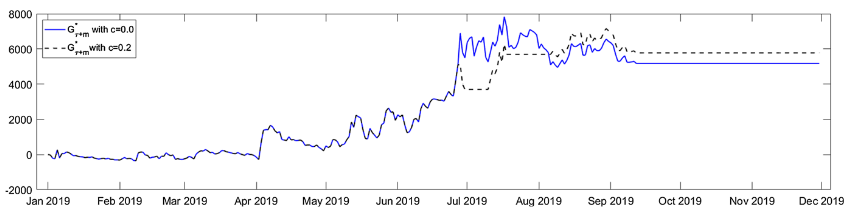
\includegraphics[width=0.8\textwidth]{background/Images/gains.png}
    \caption{Net gains taking transaction fees into account~\cite{Figa-TalamancaGianna2021Cdff}}
    \label{fig:gains}
\end{figure}

\noindent Overall although there have been countless studies that explored statistical analysis of arbitrage opportunities on centralised exchanges, little attention has been given to investigating such opportunities on decentralised exchanges. Profitable methods like mean reversion, mean reversion utilizing the Kalman filter, and analyzing cointegrated cryptocurrencies have been identified in centralised exchange settings. Consequently, it would be intriguing to explore whether these findings hold true when applied to decentralised exchanges.
